\subfloat{
  \begin{tikzpicture}
    \begin{axis}[trim axis left, trim axis right, width=0.9\textwidth, height=0.4\textheight,
      xlabel={Time (sec)},
      ylabel={ParticleWeightSum},
      legend entries={with recovery, without recovery},
      grid = major]
      \addplot [red, mark=x] table[col sep=semicolon, x=timestamp, y=normalizedWeightSum] {csv/F-Foyer2_F007-F023-F007_kidnapping/ParticleWeight_withRecovery.csv};
      \addplot [blue, mark=x] table[col sep=semicolon, x=timestamp, y=normalizedWeightSum] {csv/F-Foyer2_F007-F023-F007_kidnapping/ParticleWeight_withoutRecovery.csv};
    \end{axis}
  \end{tikzpicture}
}

\subfloat[with recovery] {
  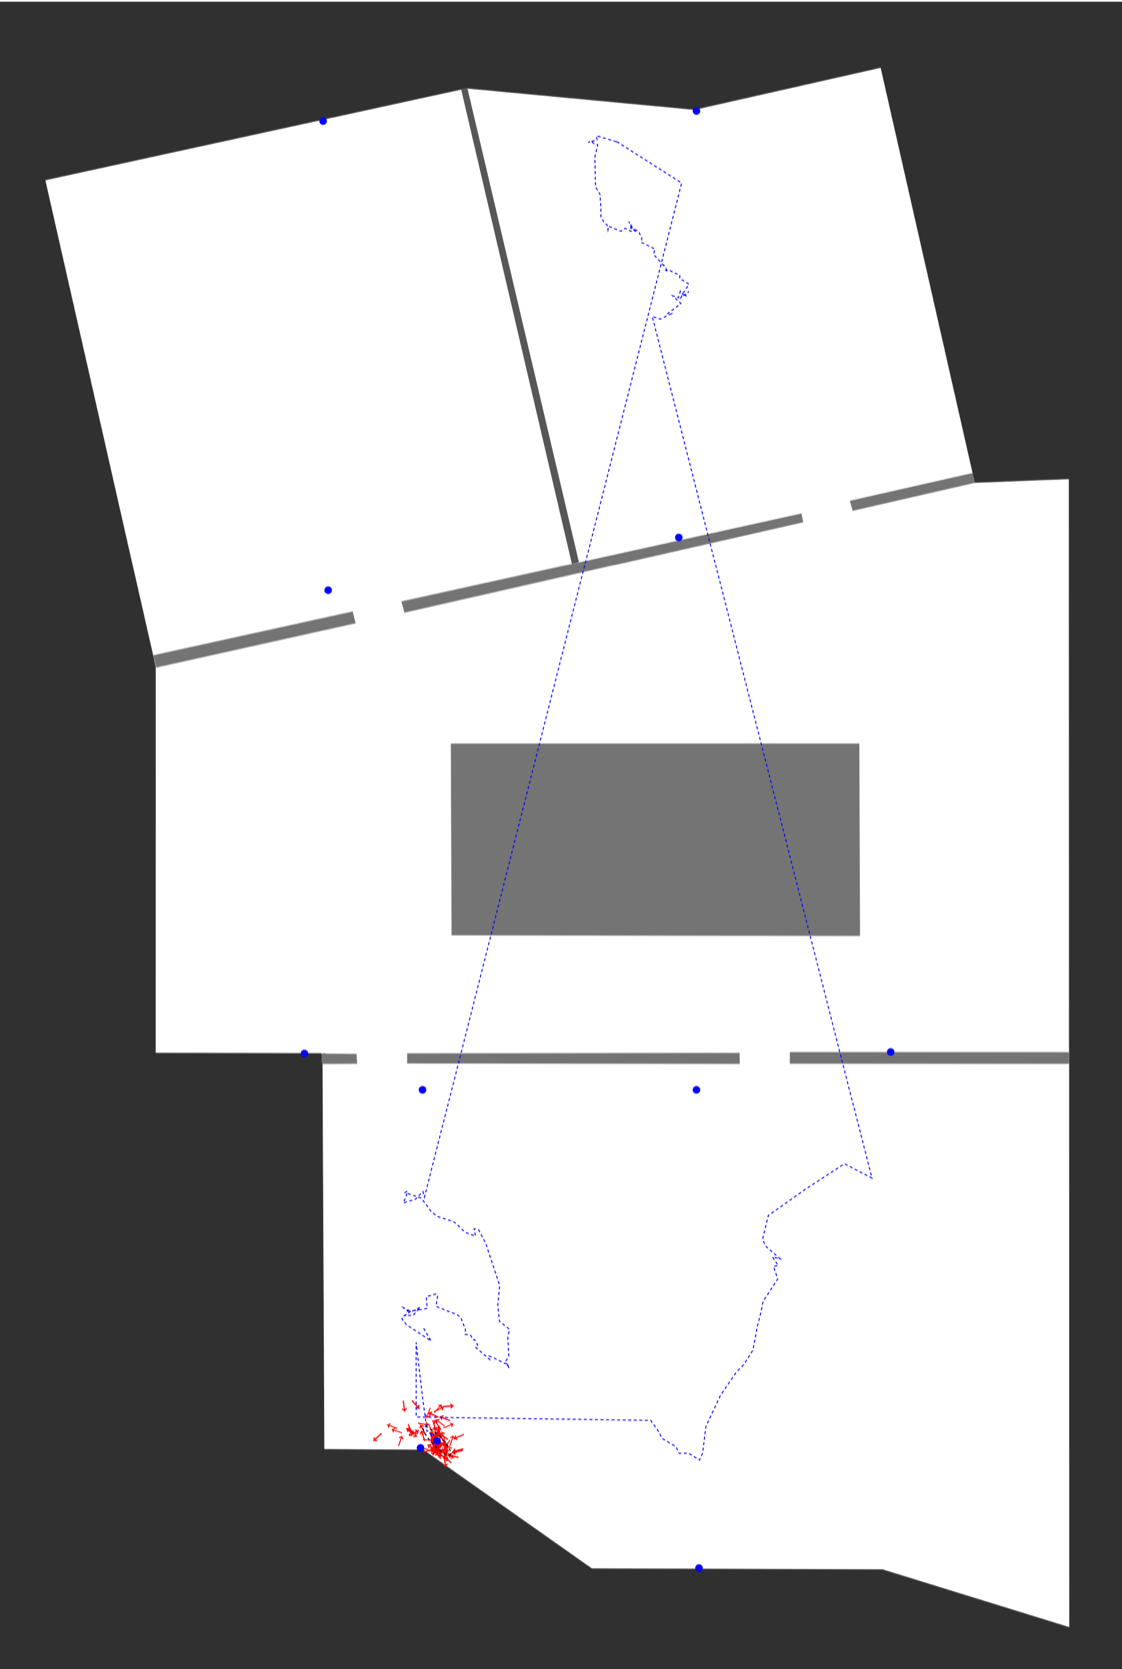
\includegraphics[height=0.5\textheight]{figures/algo_withRecovery}
  \label{fig:algo_recovery_withRecovery}
}
\subfloat[without recovery] {
  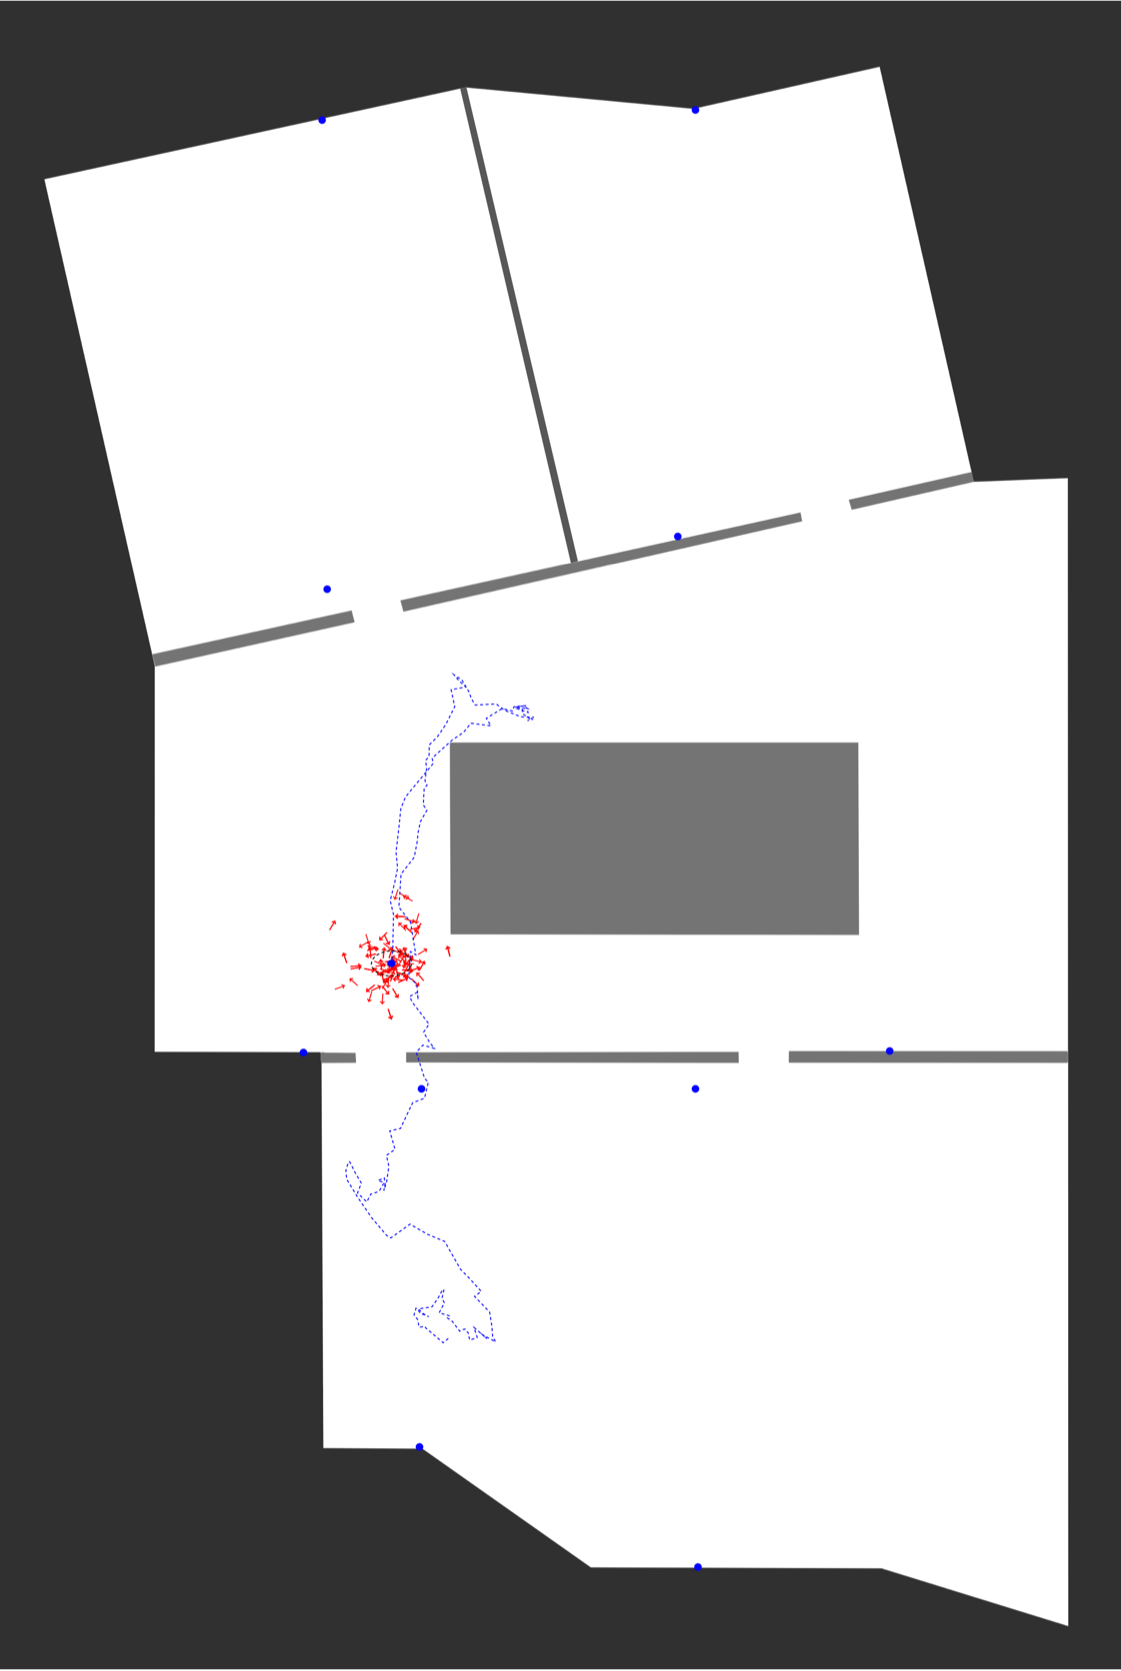
\includegraphics[height=0.5\textheight]{figures/algo_withoutRecovery}
  \label{fig:algo_recovery_withoutRecovery}
}
